% ------------------------------------------------------------------------------
% Este fichero es parte de la plantilla LaTeX para la realización de Proyectos
% Final de Grado, protegido bajo los términos de la licencia GFDL.
% Para más información, la licencia completa viene incluida en el
% fichero fdl-1.3.tex

% Copyright (C) 2012 SPI-FM. Universidad de Cádiz
% ------------------------------------------------------------------------------
En esta sección se tratan los aspectos relacionados con la con la implementación
del sistema y su codificación. Para ello se describen las herramientas software
y hardware utilizadas en el desarrollo, y la estructura del código fuente. 

\section{Entorno de construcción}

\begin{description}
   \item[Entorno de desarrollo (IDE):] Geany 1.24 
   \item[Lenguaje de programación:] C++ 03
   \item[Compilador:] GCC 4.9
   \item[Configuración automática:] Autoconf 2.69
   \item[Construcción automática:] Automake 1.14
   \item[Gestión de dependencias:] Make 4.0
   \item[Control de versions:] Subversion 1.8.10
   \item[Generador de analizador léxico:] Flex 2.5.39
   \item[Generador de analizador sintáctico:] Bison 3.0.4
   \item[Depurador:] GDB  7.7.1
   \item[Bibliotecas de desarrollo] \hfill 
      \begin{description}
         \item[Editor de línea e histórico:] Readline 5.2
         \item[Expresiones regulares:] BoostRegex 1.55
         \item[Matemáticas:] Biblioteca estándar de C 2.19
         \item[Enlaces dinámicos:] Biblioteca del sistema GNU/Linux libdl 3.1.8
      \end{description}
   \item[Desarrollo Web] \hfill 
      \begin{description}
         \item[Programación en servidor:] PHP 5.6
         \item[Programación en cliente:] JavaScript 1.5
         \item[Estructura del contenido:] HTML5
         \item[Presentación del contenido:] CSS 3
      \end{description}
\end{description}

\section{Ficheros de código fuente}
El sistema software se constituye de una serie de módulos o componentes en forma de ficheros, 
cada uno de los cuales contiene las estructuras de programación y el código fuente necesario
para implementar cada una de las funcionalidades del sistema.

\begin{description}
\item [interpreter:] Interprete.
\item [lshScanner:] Analizador léxico.
\item [lshParser:] Analizador sintáctico.
\item [error:] Sistema de errores.
\item [plugins:] Sistema de extensiones.
\item [run/runTree:] Abstracción de nodo ejecutable.
\item [run/expNode:] Abstracción de nodos ejecutables expresiones.
\item [run/symbols:] Estructura de datos tabla de símbolos.
\item [run/sTable:] Gestión de tabla de de símbolos y definiciones.
\item [run/typeNode:] Nodos ejecutables para cada tipo de dato.
\item [run/numData:] Representación interna de datos numéricos.
\item [run/stmtNode:] Nodos ejecutables sentencias de control.
\item [run/operatorBaseNode:] Nodos ejecutables operadores básicos.
\item [run/operatorLogicNode:] Nodos ejecutables operadores lógicos.
\item [run/operatorArithNode:] Nodos ejecutables operadores aritméticos.
\item [run/operatorStrNode:] Nodos ejecutables operadores sobre cadenas.
\item [run/operatorArrayNode:] Nodos ejecutables operadores sobre arrays.
\item [run/operatorRegexpNode:] Nodos ejecutables operadores sobre expresiones regulares.
\item [run/operatorDateNode:] Nodos ejecutables operadores sobre fechas y tiempo.
\item [run/operatorFileNode:] Nodos ejecutables operadores sobre ficheros.
\item [run/operatorProcessNode:] Nodos ejecutables operadores sobre procesos.
\end{description}

A continuación se describen las dependencias entre ficheros mediante una serie de paquetes que contienen diagramas de componentes.
Este aspecto del sistema queda completamente descrito mediante la combinación de estos paquetes.

\begin{center}
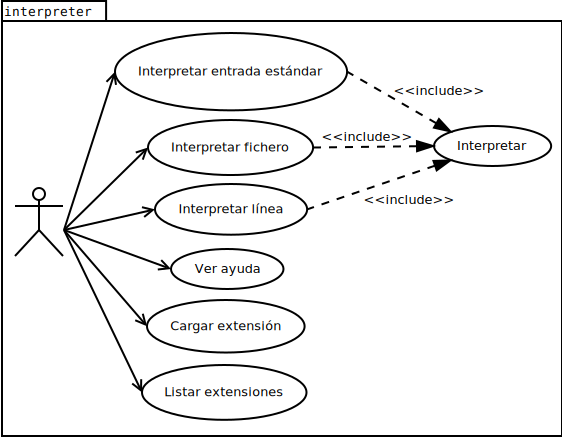
\includegraphics[scale=0.3]{dev/interpreter.png} 
\captionof{figure}{Ficheros intérprete}
\end{center}
\pagebreak

\begin{multicols}{2}
\begin{center}
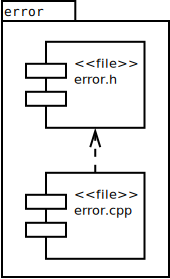
\includegraphics[scale=0.3]{dev/error.png} 
\captionof{figure}{Ficheros error}
\end{center}
\begin{center}

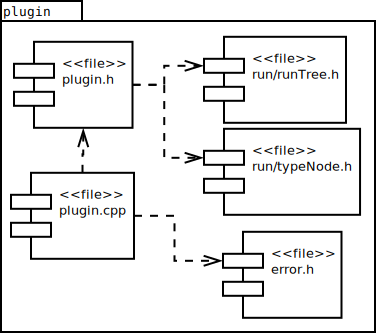
\includegraphics[scale=0.3]{dev/plugin.png} 
\captionof{figure}{Ficheros plugin}
\end{center}
\end{multicols}

\begin{multicols}{2}
\begin{center}
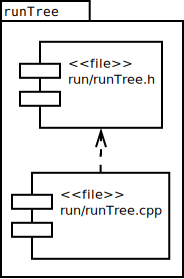
\includegraphics[scale=0.3]{dev/runTree.png} 
\captionof{figure}{Ficheros runTree}
\end{center}
\begin{center}

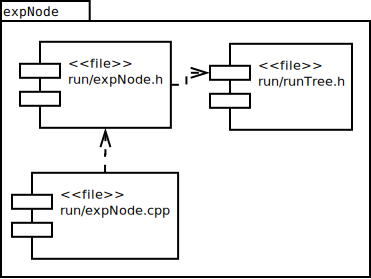
\includegraphics[scale=0.3]{dev/expNode.png} 
\captionof{figure}{Ficheros expNode}
\end{center}
\end{multicols}

\begin{multicols}{2}
\begin{center}
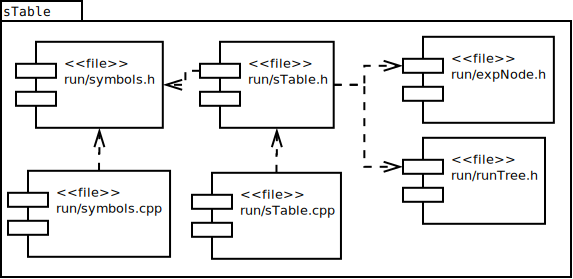
\includegraphics[scale=0.3]{dev/sTable.png} 
\captionof{figure}{Ficheros sTable}
\end{center}
\begin{center}

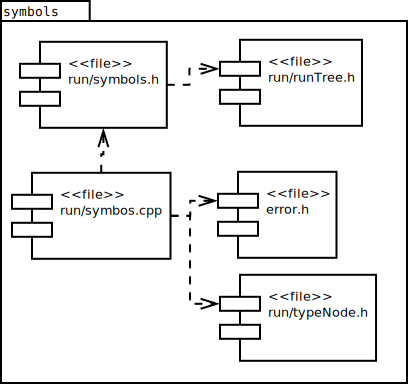
\includegraphics[scale=0.3]{dev/symbols.png} 
\captionof{figure}{Ficheros symbols}
\end{center}
\end{multicols}
\pagebreak

\begin{multicols}{2}
\begin{center}
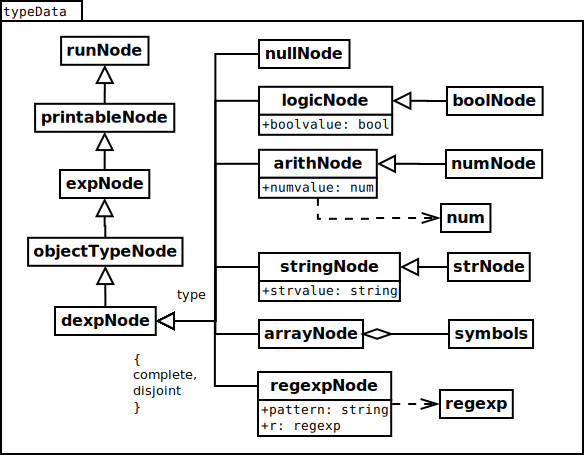
\includegraphics[scale=0.3]{dev/typeData.png} 
\captionof{figure}{Ficheros typeData}
\end{center}
\begin{center}

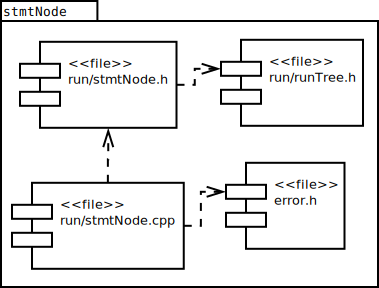
\includegraphics[scale=0.3]{dev/stmtNode.png} 
\captionof{figure}{Ficheros stmtNode}
\end{center}
\end{multicols}

\begin{multicols}{2}
\begin{center}
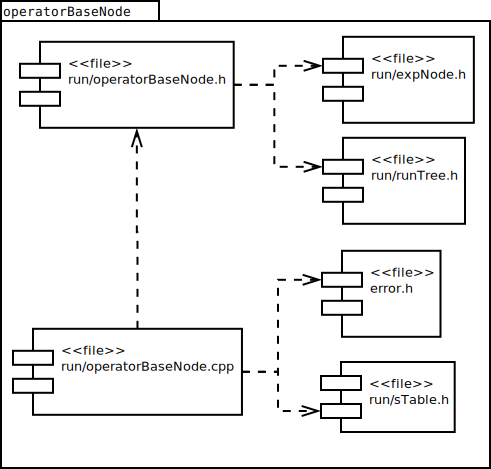
\includegraphics[scale=0.3]{dev/operatorBaseNode.png} 
\captionof{figure}{Ficheros operatorBaseNode}
\end{center}
\begin{center}

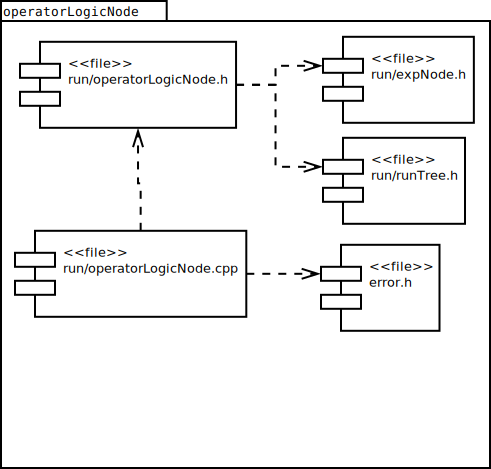
\includegraphics[scale=0.3]{dev/operatorLogicNode.png} 
\captionof{figure}{Ficheros operatorLogicNode}
\end{center}
\end{multicols}

\begin{multicols}{2}
\begin{center}
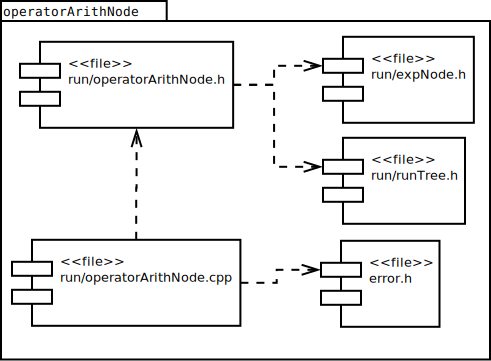
\includegraphics[scale=0.3]{dev/operatorArithNode.png} 
\captionof{figure}{Ficheros operatorArithNode}
\end{center}
\begin{center}

\includegraphics[scale=0.3]{dev/operatorStrNode.png} 
\captionof{figure}{Ficheros}
\end{center}
\end{multicols}

\begin{multicols}{2}
\begin{center}
\includegraphics[scale=0.3]{dev/operatorArrayNode.png} 
\captionof{figure}{Ficheros operatorArrayNode}
\end{center}
\begin{center}

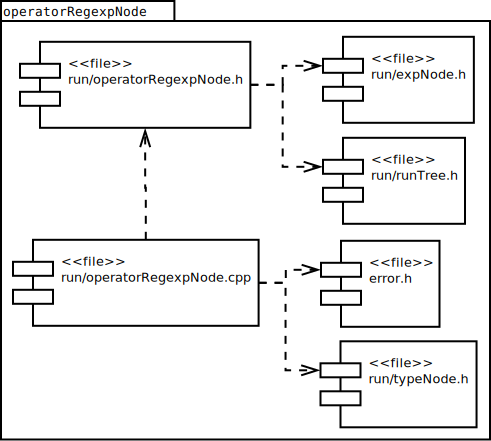
\includegraphics[scale=0.3]{dev/operatorRegexpNode.png} 
\captionof{figure}{Ficheros operatorRegexpNode}
\end{center}
\end{multicols}

\begin{multicols}{2}
\begin{center}
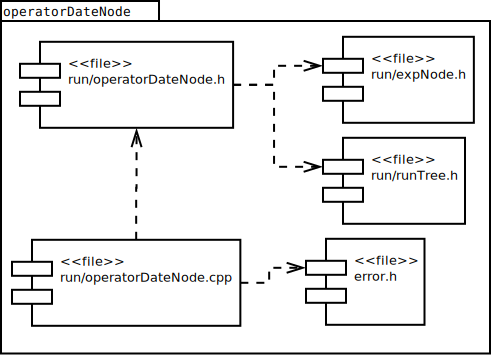
\includegraphics[scale=0.3]{dev/operatorDateNode.png} 
\captionof{figure}{Ficheros operatorDatteNode}
\end{center}
\begin{center}
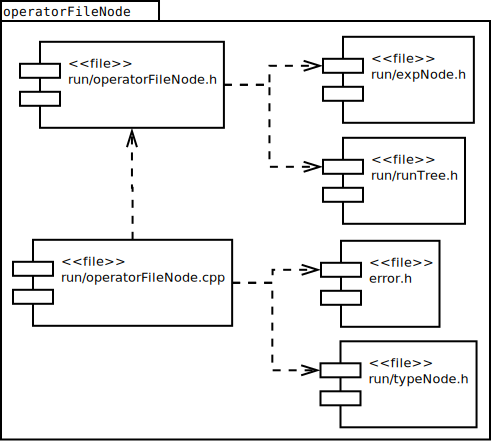
\includegraphics[scale=0.3]{dev/operatorFileNode.png} 
\captionof{figure}{Ficheros operatorFileNode}
\end{center}
\end{multicols}


%~ \begin{multicols}{2}
\begin{center}
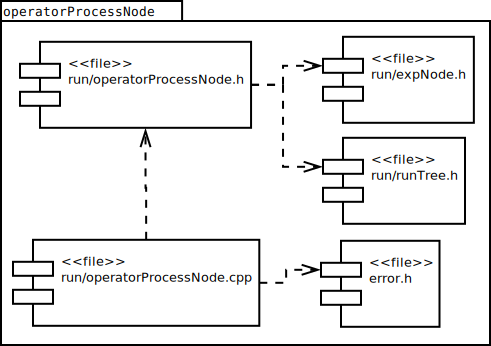
\includegraphics[scale=0.3]{dev/operatorProcessNode.png} 
\captionof{figure}{Ficheros operatorProcessNode}
\end{center}
%~ \end{multicols}

\section{Código fuente}
En esta sección se presentan extractos de código fuentes pertenecientes al intérprete OMI. Se ha tomado los métodos ``run'' de nodos significativos dado que es el método que 
se encarga de producir el significado semántico. Se presentan nodos relativos al acceso a la tabla de símbolos variables, a la asignación y la operación suma debido a su importancia y su simplicidad. 

\subsection{Acceso a variable}

%~ \begin{lstlisting}[language=cpp]
\begin{lstlisting}[language=cpp]
void idNode::run (bool resolvkey) {
   #if JSON==1
      interpreter::to_jsonRun(this);
   #endif
   sTable *table_ = sTable::sTable_use;
   refNode *str = new refNode(id_);
   exist_ = table_->exist (str);
   ref_ = table_->access (str);
   delete str;
   runNode *val = ref_->getRef();
   refNode * key = NULL;
   ref_ = refNode::resolved (val);
   if (privateNode::is)
      table_->setPrivate(new refNode (id_));
   if (!ref_->isprivate_)
      ref_->isprivate_ = privateNode::is;
   #if JSON==1
         interpreter::to_jsonSetValue(this, val);
   #endif
}
\end{lstlisting}
\captionof{lstlisting}{Código acceso a variable}

\subsection{Asignación}
\begin{lstlisting}[language=cpp]
void asigNode::run () {
   runNode *node_aux = node2_, *nodeR_ = NULL;
   #if JSON==1
      interpreter::to_jsonRun(this);
   #endif
   ref_ = NULL;
   nexpNode::resolvedRef (node_aux);
   #if JSON==1
      if (node2_ != node_aux)
         interpreter::to_jsonRun(this);
   #endif
   if (!(bool)dynamic_cast<functionNode*>(node_aux) && node2_ == node_aux) {
      node_aux->run();
      #if JSON==1
         interpreter::to_jsonRun(this);
      #endif
   }
   nodeR_ = this->isRefNode (node_aux)?node_aux:expNode::clone (node_aux);
   noderef(nodeR_);
   #if JSON==1
      interpreter::to_jsonSetValue(this, nodeR_);
   #endif
   setValue (nodeR_);
}
\end{lstlisting}
\captionof{lstlisting}{Código asignación}
\pagebreak

\subsection{Operación suma}
\begin{lstlisting}[language=cpp]
void addNode::run () {
   #if JSON==1
      interpreter::to_jsonRun(this);
   #endif         
   runNode* op1 = node1_;
   runNode* op2 = node2_;
   nexpNode::resolved (op1);
   #if JSON==1
      interpreter::to_jsonRun(this);
   #endif      
   nexpNode::resolved (op2);
   #if JSON==1
      interpreter::to_jsonRun(this);
   #endif         
   numvalue_ = addNode::do_add (op1, op2);
   #if JSON==1
      interpreter::to_jsonSetValue(this, numvalue_);
   #endif
}
\end{lstlisting}
\captionof{lstlisting}{Código operación suma}
